% Ubah kalimat sesuai dengan judul dari bab ini
\chapter{TINJAUAN PUSTAKA}

% Ubah konten-konten berikut sesuai dengan yang ingin diisi pada bab ini

\section{\textit{Machine Learning}}

% Contoh input gambar dengan format *.jpg
% \begin{figure} [ht] \centering
%   % Nama dari file gambar yang diinputkan
%   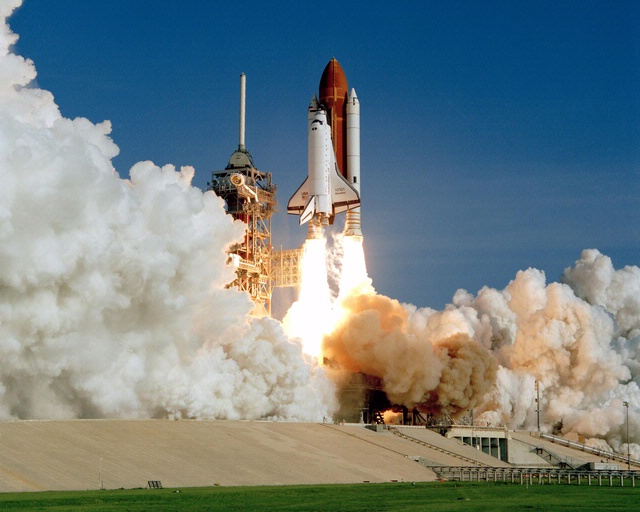
\includegraphics[scale=0.3]{gambar/space-shuttle.jpg}
%   % Keterangan gambar yang diinputkan
%   \caption{Peluncuran pesawat luar angkasa Discovery \citep{DiscoverySpaceShuttle}}
%   % Label referensi dari gambar yang diinputkan
%   \label{fig:SpaceShuttle}
% \end{figure}

\textit{Machine Learning} (ML) merupakan sebuah cabang dari \textit{Artificial Intelligence} (kecerdasan buatan) yang memungkinkan sistem
komputer untuk belajar langsung dari contoh, data, dan pengalaman yang didapatkannya. Dengan begitu, ML dapat melakukan algoritma kompleks tanpa intruksi / program manual yang dibuat oleh manusia.

Salah satu ciri khas dari ML adalah adanya proses \textit{training} (pembelajaran). Oleh karena itu, ML membutuhkan data untuk dipelajari yang disebut sebagai \textit{data training}. Setelah berhasil melakukan \textit{training}, maka ML dapat melakukan proses klasifikasi atau prediksi terhadap data baru yang diberikan sesuai dengan hasil \textit{training} yang telah dilakukan.

Klasifikasi adalah metode dalam ML yang digunakan oleh mesin untuk memilah atau mengklasifikasikan objek berdasarkan ciri tertentu sebagaimana manusia mencoba membedakan benda satu dengan yang lain\citep{shalev-shwartz_ben-david_2014}. Sedangkan prediksi digunakan oleh mesin untuk menerka keluaran dari suatu data masukan. 
% Contoh penggunaan referensi dari gambar yang diinputkan
% \emph{Discovery}, Gambar \ref{fig:SpaceShuttle}, merupakan \lipsum[17][1-9]

\section{\textit{Deep Learning}}
\textit{Deep Learning} (DL) adalah salah satu bidang yang muncul dari penelitian ML.
DL memungkinkan model komputasi yang tersusun dari banyak lapisan pemrosesan pembelajaran untuk mempelajari representasi dari data dengan berbagai level.
DL dapat menemukan struktur sulit yang terdapat di dalam kumpulan data yang besar dengan menggunakan algoritma \textit{backpropagation} \citep{DBLP:journals/corr/ZhangBHRV16}.
Struktur yang didapatkan menunjukkan paramater internal apa yang harus diubah oleh mesin agar dapat menghitung representasi di setiap \textit{layer} berdasarkan representasi dari \textit{layer} sebelumnya.

DL juga melakukan pendekatan dalam penyelesaian masalah dengan menggunakan konsep hierarki.
Dengan konsep tersebut, komputer mampu mempelajari sebuah konsep yang kompleks dengan menggabungkan
konsep-konsep yang lebih sederhana.

\section{\textit{Convolutional Neural Network}}
\textit{Convolutional Neural Network} (CNN) merupakan variasi dari \textit{Multilayer Perceptron} yang terinspirasi dari jaringan saraf manusia\citep{CNN2017}.
Nama \textit{convolutional neural network} dapat menggambarkan bahwa jaringan ini menggunakan operasi matematika yang disebut konvolusi.
CNN merupakan pengembangan dari \textit{artificial neural network} yang saat ini diklaim sebagai model terbaik untuk memecahkan masalah
seputar \textit{object recognition} dan \textit{detection}.

Secara teknis, CNN adalah arsitektur yang bisa di-\textit{training}
dan terdiri dari beberapa tahap. Input dan output dari masingmasing tahap berupa \textit{array} yang disebut \textit{feature map} atau peta fitur. Output dari masing-masing tahap adalah \textit{feature map} hasil pengolahan dari semua lokasi pada input. Struktur CNN dibangun dari tiga jenis layer utama yaitu \textit{convolution layer}, \textit{pooling layer}, dan \textit{activation function} \citep{CNN2017}.

\section{\textit{Computer Vision}}
\textit{Computer vision} adalah suatu cara menganalisis citra dan video oleh komputer untuk memperoleh hasil sebagaimana yang bisa dilakukan manusia.
Pada hakikatnya, \textit{computer vision{ mencoba meniru cara kerja sistem visual manusia \citep{IJAIR42}. Manusia melihat objek dengan indra penglihatan (mata), lalu citra objek diteruskan ke otak untuk diinterpretasi sehingga manusia mengerti objek apa yang tampak dalam pandangan matanya.
Hasil interpretasi ini kemudian digunakan untuk pengambilan keputusan.
Pada komputer, hal ini dilakukan dengan melakukan penangkapan citra atau video melalui kamera, lalu dilakukan proses analisis terhadap gambar tersebut. Hasil analisis digunakan untuk melakukan keputusan-keputusan yang dibuat berdasarkan kondisi
citra atau video yang ditangkap oleh kamera. \textit{Computer vision} dibuat agar dapat membantu manusia melakukan proses pengamatan
dan pengambilan keputusan yang sulit jika dilakukan dalam kondisi yang spesifik.

\section{\textit{Image Processing}}
Di dalam bidang komputer terdapat tiga bidang studi yang
berkaitan dengan data citra, namun dengan tujuan yang berbeda\citep{Umam2016},
yaitu:

\begin{enumerate}
  \item Pengenalan Pola
    
  Pengenalan pola mengelompokkan data numerik dan simbolik (termasuk citra) secara otomatis oleh mesin (dalam hal ini
  komputer). Tujuan pengelompokan adalah untuk mengenali
  suatu objek di dalam citra. Manusia bisa mengenali objek
  yang dilihatnya karena otak manusia telah belajar mengklasifikasi objek-objek di alam sehingga mampu membedakan suatu objek dengan objek lainnya. Kemampuan sistem visual
  manusia inilah yang dicoba ditiru oleh mesin. Komputer menerima masukan berupa citra objek yang akan diidentifikasi,
  memproses citra tersebut, dan memberikan keluaran berupa
  deskripsi objek di dalam citra.

  \item Grafika Komputer
  
  Grafika Komputer bertujuan menghasilkan citra dengan primitif-primitif geometri seperti garis, lingkaran dan sebagainya. Primitif-primitif geometri tersebut memerlukan data deskriptif untuk
  melukis elemen-elemen gambar. Contoh data deskriptif adalah koordinat titik, panjang garis, jari-jari lingkaran, tebal
  garis, warna, dan sebagainya. Grafika komputer memainkan peranan penting dalam visualisasi dan \textit{virtual reality}.

  \item Pengolahan Citra
    
  Pengolahan Citra bertujuan memperbaiki kualitas citra agar
  mudah diinterpretasi oleh manusia atau mesin (komputer).
  Teknik-teknik pengolahan citra mentransformasikan citra menjadi citra lain. Jadi, masukannya adalah citra dan keluarannya
  juga citra, namun dengan kualitas yang lebih baik daripada
  citra masukan.
\end{enumerate}

\section{\textit{FaceNet}}
\textit{FaceNet} menggunakan (CNN). CNN di \textit{training} sedemikian rupa sehingga jarak kuadrat L2 antara \textit{vector embeddings} sesuai dengan kesamaan wajah.
Gambar yang digunakan untuk \textit{training} telah diskalakan sebelumnya, lalu diubah dan dipotong di sekitar area wajah.
Aspek penting lain dari \textit{FaceNet} adalah \textit{loss function}nya. FaceNet menggunakan \textit{triplet loss function} dibandingkan model-model lain yang hanya menggunakan \textit{single loss function}.
Untuk menghitung \textit{triplet loss}, membutuhkan 3 gambar sebagai acuan yaitu \textit{anchor}, positif dan negatif\citep{Facenet2015}.

\section{Docker}
Docker adalah layanan yang menyediakan kemampuan untuk mengemas dan menjalankan sebuah aplikasi dalam sebuah lingkungan terisolasi yang disebut dengan \textit{container}.
Dengan adanya isolasi dan keamanan yang memadai memungkinkan kamu untuk menjalankan banyak container di waktu yang bersamaan pada host tertentu.
Docker diperkenalkan pada tahun 2013 oleh Solomon Hykes pada acara PyCon. Beberapa bulan setelahnya docker secara resmi diluncurkan, tepatnya pada tahun 2014.
\subsection{Fitur - fitur Docker}
\begin{itemize}
  \item Docker engine
  
  Docker engine adalah \textit{core} dari docker, digunakan untuk membuat \textit{image} dan \textit{container}.

  \item Docker Hub
  
  Docker hub adalah \textit{registry} yang berisikan kumpulan dari berbagai \textit{image} yang disimpan di \textit{data center} milik docker.
  Dengan menggunakan docker hub ini memungkinkan pengguna untuk dapat mengumpulkan dan mendapatkan \textit{image}.  

  \item Docker Compose
  
  Docker compose adalah salah satu fitur unggulan yang berfungsi untuk menjalankan beberapa \textit{container} atau disebut \textit{multi-container} sehingga dapat menghemat banyak waktu.

\end{itemize}

\subsection{Kelebihan}
\begin{itemize}
  \item Konfigurasi yang sederhana
  
  Docker memiliki konfigurasi yang cukup sederhana dan dapat disesuaikan dengan kebutuhan aplikasi yang sedang dikembangkan.
  Dengan beberapa kode, docker akan membuat \textit{environment} sendiri yang berbeda dengan \textit{environment} dari server utama.

  \item Tingkat keamanan yang baik
  
  Docker memastikan aplikasi yang sedang berjalan tidak dapat memengaruhi \textit{container}.
  Selain itu, ia juga memiliki fitur keamanan lain seperti pengaturan OS \textit{host mount} dengan akses \textit{read-only} sehingga tidak akan mengubah konfigurasi apa pun, kecuali \textit{user} yang memiliki akses secara penuh.

  \item Dapat dijalankan pada platform \textit{cloud}
  
  Docker dapat dijalankan pada \textit{platform cloud}, sehingga penggunanya akan lebih fleksibel dalam melakukan \textit{porting} aplikasi.

  \item \textit{Debugging} yang lebih cepat
  
  Waktu yang dibutuhkannya untuk \textit{debugging} docker \textit{container} tergolong cepat, yaitu sekitar satu menit saja untuk melakukan proses \textit{debug} pada Sandbox.

\end{itemize}

\subsection{Shell Linux}

Shell adalah program yang menghubungkan \textit{user} dengan sistem operasi dalam hal ini kernel (inti sistem operasi).
Umumnya, shell menyediakan \textit{prompt} sebagai \textit{user interface}, tempat dimana user meng\textit{input} perintah-perintah yang diinginkan baik berupa perintah internal shell (\textit{internal command}),
ataupun perintah eksekusi suatu file progam (\textit{external command}), selain itu shell memungkinkan \textit{user} menyusun sekumpulan perintah pada sebuah atau beberapa \textit{file} untuk dieksekusi sebagai program.
Tidak seperti sistem operasi lain yang hanya menyediakan 1 atau 2 shell, sistem operasi dari keluarga unix misalnya linux sampai saat ini dilengkapi oleh banyak shell dengan kumpulan perintah yang sangat banyak, sehingga memungkinkan pemakai memilih shell mana yang paling baik untuk membantu menyelesaikan pekerjaannya, atau dapat pula berpindah-pindah dari shell yang satu ke shell yang lain dengan mudah.

\section{Vue JS}
Vue JS adalah salah satu \textit{framework} atau \textit{library} dari JavaScript yang digunakan untuk untuk membuat tampilan (\textit{interface}) pada website agar tampak lebih interaktif.
Fungsi lain dari Vue JS adalah membuat SPA (\textit{Single Page Application}). Apabila digunakan pada arsitektur MVC (\textit{Model – View – Controller}), maka framework ini menempati pada posisi View yang berjalan di sisi \textit{front end}.
Tugas utama dari \textit{framework} ini adalah mengirim dan menerima data, kemudian membuat tampilan UI (\textit{User Interface}) yang menarik. \textit{Framework} ini juga sangat mudah untuk diintegrasikan dengan \textit{library} yang lain.
Jika diimplementasikan pada komponen HTML, maka Vue JS menggunakan ID, \textit{class}, atau \textit{name} untuk menginisialisasikannya.
\textit{Framework} ini mengalami perkembangan yang pesat, bahkan beberapa perusahaan besar menggunakannya, sebagai contoh Google dan Adobe. Terlepas dari itu, Vue JS pertama kali dikembangkan pada tahun 2013 oleh Evan You yang sebelumnya bekerja di Google dengan menggunakan AngularJS.
Hal itulah yang melatarbelakangi seorang Evan You mengembangkan sebuah library yang lebih ringan daripada AngularJS.

\subsection{Fitur - fitur Vue JS}
\begin{itemize}
  \item \textit{Components}
  
  Fitur \textit{components} digunakan untuk membuat berbagai elemen pada HTML secara \textit{custom}. Elemen \textit{custom} ini juga dapat digunakan secara berulang – ulang.

  \item \textit{Computed Properties}
  
  Fitur \textit{computed properties} digunakan untuk melihat setiap perubahan yang terjadi dalam elemen \textit{user interface} tanpa harus melakukan penambahan kode di dalamnya.

  \item \textit{Data Binding}
  
  \textit{Data binding} digunakan untuk memanipulasi dan memberikan nilai (\textit{value}) pada atribut HTML. Sebagai contoh, mengubah style dengan menggunakan bantuan \textit{binding directives}, yaitu V-Bind.

  \item \textit{Directives}
  
  Fitur \textit{directives} berfungsi untuk melakukan berbagai aksi (\textit{action}) pada antarmuka \textit{front end website}. Contoh perintah bawaan yang digunakan adalah v-if, v-else, v-model, dan lainnya.

  \item \textit{Event Handling}
  
  \textit{Event handling} atau v-on yang berfungsi sebagai atribut yang dapat ditambahkan ke dalam suatu elemen DOM untuk sebuah \textit{event} pada Vue JS.

  \item \textit{Lightweight}
  
  Fitur \textit{lightweight} yang digunakan untuk membuat menjadi lebih sederhana, akan tetapi masih tetap cepat dan \textit{powerful}.

  \item \textit{Routing}
  
  Fitur \textit{routing} mempunyai kegunaan sebagai perantara atau penghubung antar setiap halaman. Fitur ini memiliki kelebihan dalam membuat aplikasi \textit{single-page}, cukup dengan menggunakan satu \textit{file} HTML saja.

  \item \textit{Template}
  
  Fitur \textit{templates} berfungsi untuk menghubungkan DOM dengan \textit{data instance} pada Vue JS, yang nantinya akan mengkompilasi \textit{template} menjadi fungsi \textit{DOM Render Virtual}.

  \item \textit{Virtual DOM}
  
  DOM atau kependekan dari \textit{Document Object Model} merupakan suatu \textit{interface} yang memudahkan dalam mengakses atau menambah konten pada suatu dokumen. Fitur dari \textit{Virtual DOM} berfungsi untuk menyimpan perubahan dokumen pada replika DOM, sehingga dapat di-- \textit{review} lebih cepat setiap perubahannya.

  \item \textit{Watchers}
  
  Fitur \textit{watchers} memiliki fungsi untuk dapat menangani setiap perubahan data, sehingga mampu untuk membuat kode menjadi sederhana dan cepat.



\end{itemize}

\section{Celery}

Celery adalah system penggelola antrian (\textit{task-queue}) yang menangani distribusi \textit{task} pada \textit{workers}.
Celery membuat menajemen task asinkron menjadi mudah, aplikasi hanya perlu mempublish pesan ke broker seperti RabbitMQ.
Celery dapat digunakan dalam berbagai konfigurasi.
Salah satunya yang sering digunakan adalah mengelola task asinkron yang panjang pada sebuah aplikasi,
contohnya seperti menangani data video yang diambil per \textit{frame} dari sebuah aplikasi.
% \section{Gravitasi}

% Gravitasi merupakan \lipsum[18][1-10]

% \subsection{Hukum Newton}

% % Contoh penggunaan referensi dari pustaka
% Newton \citep{Newton1687} pernah merumuskan bahwa \lipsum[19]
% % Contoh penggunaan referensi dari persamaan
% Kemudian menjadi persamaan seperti pada persamaan \ref{eq:FirstNewtonLaw}.

% % Contoh pembuatan persamaan
% \begin{equation}
%   % Label referensi dari persamaan yang dibuat
%   \label{eq:FirstNewtonLaw}
%   % Baris kode persamaan yang dibuat
%   \sum \mathbf{F} = 0\; \Leftrightarrow\; \frac{\mathrm{d} \mathbf{v} }{\mathrm{d}t} = 0.
% \end{equation}

% \subsection{Anti Gravitasi}

% Anti gravitasi merupakan \lipsum[20]
